\documentclass[11pt]{article}
\usepackage{polski}
\usepackage[utf8]{inputenc}
\usepackage{graphicx}
\usepackage{bchart}
\begin{document}
\title{Quadratic SVM}
\author{Katarzyna Krzywonos \\ Aleksandra Lubzińska}
\date{12 luty 2017}
\maketitle


\begin{center}

\includegraphics{logo_agh}\\
\vspace{20mm}
{\LARGE Klasyfikacja uderzeń serca klasyfikatorem Quadratic SVM}\\

\end{center}

\newpage
\tableofcontents
\vspace{10mm}
\newpage
\section*{Cel projektu}
Celem projektu była klasyfikacja rytmu serca przy użyciu Maszyny wektorów nośnych (ang. Support Vector Machine). Do realizacji tego zadania użyto algorytmu SMO (ang. Sequential Minimal Optimization). Algorytm tez został opracowany przez Johna Platt w 1998 roku i oparty jest na QP (ang. Quadratic Programming).

\section{Wstęp teporetyczny}
\subsection{SVM}
SVM (ang. support vector machine), czyli maszyna wektorów nośnych
(wspierających), zaliczana jest do technik nadzorowanych, które analizują dane i rozpoznają
ich wzorce. Ogólnym celem SVM jest określenie przynależności danego zbioru danych do
jednej z dwóch klas przez wyznaczenie granicy między dwoma zbiorami z największym
możliwym marginesem.

\begin{figure}[h] \begin{center} \ifpdf 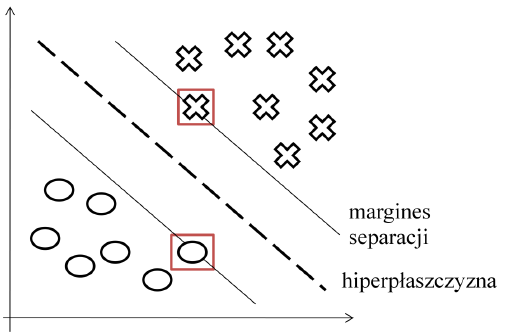
\includegraphics{SVM.png}  \textit \caption{SVM} \else 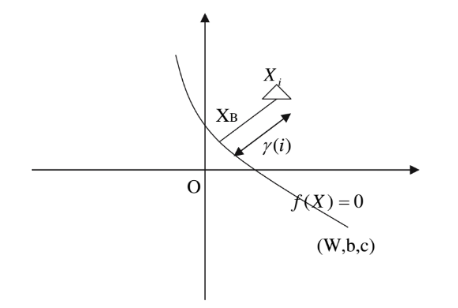
\includegraphics{3.ps} \fi \end{center} \end{figure}

\newpage
Do stworzenia takiej hiperpłaszczyzny brane są pod uwagę tylko niektóre wektory
treningowe, czyli wektory nośne, inaczej wektory podtrzymujące (ang. support vectors),
określające optymalny margines separacji.

\subsection{Quadratic SVM (ang. quadratic kernel-free non-linear support vector machine)}

Kwadratowa funkcja decyzyjna jest zdolna do rozdzielenia danych nieliniowych. 
Margines geometryczny jest równy odwrotności gradientu funkcji decyzyjnej.
Margines funkcjonalny jest równaniem funkcji kwadratowej.
\subsubsection{Kernel}
Klasy $y=\pm 1$ są kojarzone z wzorami x poprzez transformację wzorów do wektora cech $\Phi(x)$
\newline
$\widehat{y}(x) = w*\Phi+b$ 
\newline
Parametry w i b są wybierane na podstawie uruchomienia algorytmu na zestawie danych uczących $(x_1,x_2)....(x_i,x_j)$
\newline 
Paramter $\Phi$ jest dobierany indywidualnie do każdego przypadku
\newline
$w = \sum_{i=1}^{n}\alpha_i*\Phi_i $
\newline
$\widehat{y}(x) =  \sum_{i=1}^{n}\alpha_i*K(x,x_i)+b$
\newline
Funkcja Kernel K(x,y) rezprezentuje iloczyn skalarny $\Phi(x)'\Phi(y) $. To wyrażenie jest przydatne zwłaszcza wtedy, gdy duża wartość współczynników $\alpha_i$ jest równa 0. Wówczas te współczynniki, które są rózne od zera nazywane są wektorami wspierającymi. 

\subsubsection{Quadratic Programming}
QP opisuje problem optymalizacji (min lub max) kwadratową funkcją wielu zmiennych podlegających liniowym ograniczeniom. Wypukłość funkcji jest wykorzystywana do optymalizacji, ponieważ ma tylko jedno optimum, które jest globalnym optimum. 



$QSVM (W,b,c)$
$f(X)=\frac{1}{2}*X^T*W*X+b^T+c$
$f(X)=ct$ może przyjąć wszystkie formy hiperpłaszczyzny (hiper-elipsy, hiper-parabole..)
f(X) może być rozważana jako suma $fliniowe$ + $fnieliniowa$

\begin{figure}[h] \begin{center} \ifpdf 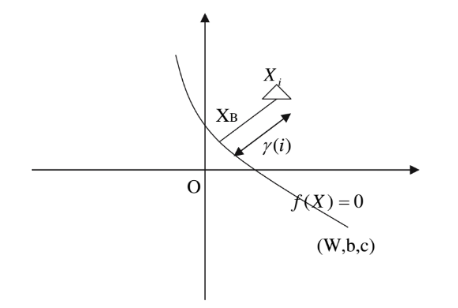
\includegraphics{3.png} \textit \caption{SMO} \else 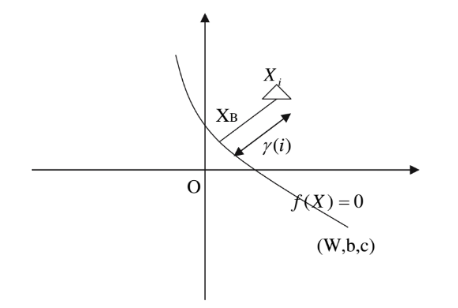
\includegraphics{3.ps} \fi \end{center} \end{figure}

\subsection{SMO}
Minimalna optymalizacja sekwencyjna SMO dekomponuje problem SVM na podproblemy, które są rozwiązywane analitycznie, lecz podproblemy są tylko dwuparametrowe. 
\subsection{Opis ogólny procedury}
Dekompozycja – wyróżnenie 2 podzbiorów parametrów: zbiór aktywny i zbiór pasywny. W każdym kroku iteracyjnym jedynie parametry aktywne są optymalizowane. Ogólną regułą algorytmów opierających się na dekompozycji jest taka optymalizacja zbioru aktywnego, by aktualne rozwiązanie było jak najbliższe maksimum globalnemu. 
Sposób wyboru aktywnego zbioru parametrów opiera się na heurystykach.
\newline
\newline
Kroki jakię są wykonywane w heurestyce
\begin{enumerate}
\item Wybór podzbioru parametrów aktywnych. 
\item Wyznaczenie rozwiązania optymalnego dla wybranych parametrów.
\item Utworzenie nowego zbioru parametrów aktywnych który składa się z
\begin{itemize}
\item Wszystkich wektorów wspierających otrzymanych w poprzednim rozwiązaniu
\item M wektorów ze zbioru pasywnego spełniającego najgorzej kryterium KKT (M – parametr systemu). 
\end{itemize}
\item W momencie spełnienia kryterium stop proces iteracyjny zostaje zatrzymany. 
\end{enumerate}

Gdy C równie jest nieskończoność wówczas mamy do czynienia z idealną separacją – pomiędzy hiperpłaszczyznami nie znajdują się zadane punkty. 
Gdy $\alpha_{i} > 0 $ to i-ty wektor jest wektorem wspierającym.
Gdy $\alpha_{i} = 0 $ to i-ty wektor może być wektorem wspierającym.
\newline
Algorytm SMO poszukuje w takim kierunku, w którym wszystkie współczynnki $\alpha$ są równe z 0 z wyjątkiem dla dwóch pojedynczych wartości 1 i -1. 

\subsection{Rozwiązanie analityczne dla dwóch punktów}
\begin{enumerate}
\item Dwoma wybranymi parametrami do zbioru aktywnego są parametry $\alpha_1$ i $ \alpha_2$. Kolejne kroki w algorytmie zaproponowanych przez Platta są następujące:
\begin{itemize}
\item $\alpha_1$ wybierany jest spośrod wszytkich paratemtrów, które nie spełniają KKT (warunki konieczne I rzędu), przy czym pierwszęnstwo mają $\alpha_1$ spełniające $ 0 < \alpha_{1} < C $. Parametr $\alpha_1$ jest to mnożnik Lagrange'a. 
\item $\alpha_2$ (drugi mnożnik Lagrange'a) musi spełniać warunek. 
\item SMO optymalizuje parę ($\alpha_1$, $\alpha_2$) i powtarza to, aż do momentu zbieżności. 
\end{itemize}
\item Wejściowe parametry spełniają warunek równościowy (są równe 0)


$ \sum_{i=1}^{l}(\alpha_{i}^{old})*y_{i}$
 
$\alpha_{1}^{old}*y_{1} + \alpha_{2}^{old}*y_{2} + \sum_{i=3}^{l}(\alpha_{i}^{old})*y_{i} = 0 $

\item Nowe wartości parametrów również muszą spełniać warunek nierównościowy
$\alpha_{1}*y_{1} + \alpha_{2}*y_{2} = \alpha_{1}^{old}*y_{1} + \alpha_{2}^{old}*y_{2} $

Po przekształceniu
$\alpha_{2} = \alpha_{1}^{old}*y_{1}*y_{2} + \alpha_{1}^{old} - \alpha_{1}*y_{1}*y_{2} $

Prosta przecina lewy bok kwadratu gdy $\alpha_{1} = 0 $
\newline Prosta przecina prawy bok kwadratu gdy $\alpha_{1} = C $

\begin{figure}[h] \begin{center} \ifpdf 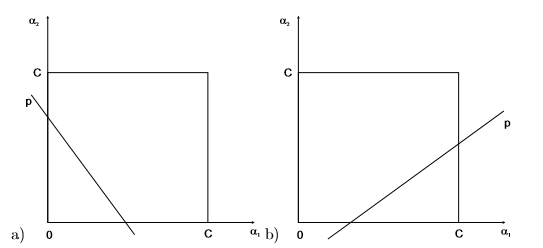
\includegraphics{1.png} \textit \caption {Rysunek przedstawia prostą p w przypadku a)o współczynniku ujemnym, w przypadku b) dodatnim.}\else 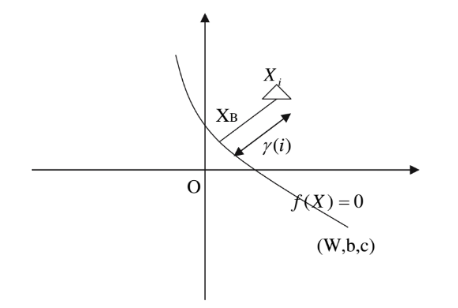
\includegraphics{3.ps} \fi \end{center} \end{figure}


Po podstawieniu otrzymuje się (gdy współczynnik kierunkowy jest ujemny (Rysunek 3. a))
\newline 
$\alpha_{2} = \alpha_{1}^{old} + \alpha_{2}^{old}$
$\alpha_{2} = \alpha_{1}^{old} + \alpha_{2}^{old}-C$
\newline Gdy współczynnik kierunkowy jest dodatni (Rysunek 3. b))
\newline
$\alpha_{2} = -\alpha_{1}^{old} + \alpha_{2}^{old}$
$\alpha_{2} = \alpha_{1}^{old} + \alpha_{2}^{old}-C$
\newline Należy pamiętać, że punkty przecięcia muszą leżeć w obrębie kwadratu. 

\item Nowe wartości parametrów muszą również spełniać warunek nierównościowy
$0\ge\alpha_{1}$ ,
$C\ge\alpha_{2}$
\item Po wykonaniu i obliczeniu parametrów  $\alpha$ ważne jest by odpowiednio ograniczyć wyniki
\newline 
Dla ułatwienia zostanie wprowadzony parametr $s=y_{1}*y_{2}$ oraz y=1 lub y=-1 
\newline 
$y_{1}*\alpha_{1} + y_{1}*\alpha_{1} = constant = \alpha_{1} + s*\alpha_{2}$
\newline
$\alpha_{1} = \gamma - s*\alpha_{2}$

Dla przypadku $s=1$   
 \newline $\alpha_{1}+\alpha_{2} = \gamma$
 \begin{itemize}
\item $\gamma > C $ max $\alpha_{2} = C $, min $ \alpha_{2} = \gamma - C$
\item $\gamma < C$  max $\alpha_{2} = 0$ ,min  $\alpha_{2} = \gamma$
\end{itemize}
Dla przypadku $s=-1$
\newline $\alpha_{1}-\alpha_{2} = \gamma$
\begin{itemize}
\item $\gamma > 0$ min $\alpha_{2} = 0 $ ,max  $\alpha_{2} = C -\gamma $
\item $\gamma < 0$ min $\alpha_{2} = -\gamma$ ,max  $\alpha_{2} = C$
\end{itemize}
W momencie gdy  $y_{1}\neq y_{2}$ 
\begin{itemize}
 \item$ U = max(0,\alpha_{2}^{old} - \alpha_{1}^{old})$
 \item$ V = max(C,C - \alpha_{1}^{old} + \alpha_{2}^{old})$
 \end{itemize}


 
W momencie gdy $y_{1}=y_{2}$
\begin{itemize}
\item$ U = max(0,\alpha_{2}^{old} + \alpha_{1}^{old} - C)$
 \item $ V = max(C, \alpha_{1}^{old} + \alpha_{2}^{old})$
 
\end{itemize}
\item Wyliczenie $E_i$ Jest to błąd, który pojawia się w momencie gdy chce się zobaczyć różnice między wyjściem a celem

$ E_i = \sum_{j=1}^{l}(\alpha_{i})*y_{j}*K(x_j,x_i)-y_i$

\item Wyliczenie $k_ij$

$\kappa = K(x_1,x_2) + K(x_2,x_2) - 2*K(x_1,x_2)$

\item Wyliczenie nowych parametrow $\alpha$ \newline
$\alpha_{2}^{unc} = \alpha_{2}^{old} + \frac{y_2*(E_1-E_2)}{\kappa}$
\newline
$\alpha_{2}$= 
\begin{itemize}
\item $V$, jesli $\alpha_{2}^{new}{unc}>V$;
\item $\alpha_{2}^{new}{unc}$, jeśli $U\ge\alpha_{2}^{new}{unc}\ge V$;
\item $U$, jeśli $U<\alpha_{2}^{new}{unc}$;
\newline
\end{itemize}
$\alpha_{new} = \alpha_{old} + y_{1}*y_{1}(\alpha_{old}-\alpha_{new})$
\newpage
\section{Implementacja rozwiązania C++}
\subsection{Zaproponowane rozwiązanie}
Patrząc pod kątem implementacji maszyny wektorów nośnych z jądrem kwadratowym metodą SMO, należy wyróżnić dwa etapy klasyfikatora : uczenie oraz predykcję/klasyfikację. W głównym programie pierwsze tworzony jest obiekt klasyfikatora QSVM, następnie jest on uczony przez wywołanie metody train(), a dopiero później następuje predykcja na próbkach testowych ( poniższy pseudokod).\\ 

\begin{tabular}{|p{11.5cm}|} \hline\noindent \#include "svm\_additional\_fnc.h"

\noindent \#include "svm\_classifier.h"

\noindent 

\noindent using std::cerr;

\noindent using std::endl;

\noindent // g{\l}\'{o}wna funkcja main

\noindent int main()

\noindent $\{$

 SVMClassifier *our\_classifier = new SVMClassifier();  // tworzenie nowego obiektu klasy SVMClassifier 

\noindent 

 clock\_t begin = clock();  // zapisanie czasu rozpocz\k{e}cia treningu w zmiennej begin typy clock\_t

 our\_classifier-$>$train(); // wywo{\l}anie metody train na obiekcie

 clock\_t train = clock(); //zapisanie czasu ko\'{n}ca treningu w zmiennej train typu clock\_t

 our\_classifier-$>$predict();// wywo{\l}anie metody predict na obiekcie

 clock\_t predict = clock(); //zapisanie czasu ko\'{n}ca predykcji do zmiennej predict typy clock\_t

 std::cout $<$$<$ "Train time:{\textbackslash}t" $<$$<$ (double(train - begin) / CLOCKS\_PER\_SEC) $<$$<$ endl;

 std::cout $<$$<$ "Predict time:{\textbackslash}t" $<$$<$ (double(predict - train) / CLOCKS\_PER\_SEC) $<$$<$ endl;

 std::cout $<$$<$ "Total time:{\textbackslash}t" $<$$<$ (double(predict - begin) / CLOCKS\_PER\_SEC) $<$$<$ endl;

 int wait;

 std::cin $>$$>$ wait; // zamkni\k{e}cie przez wpisanie liczby

\noindent 

\noindent $\}$
\\\\ \hline
\end{tabular}
\\
Pierwsze w funkcji main wywoływana jest funkcja train. Poniżej przedstawiony jest pseudokod funkcji train().\\
\begin{tabular}{|p{11.5cm}|} \hline
\noindent \textbf{Pseudokod funkcja train():}

 numChangedAlpha = 0;

 prevNumChangedAlpha = 0;

 examineAll = 1;

 rounds = 0;

 sameRounds = 0;

\noindent \textbf{while} numChangedAlpha większe od 0 lub examineAll równe True, oraz rounds $<$ maksymalnej liczby iteracji, oraz sameRounds $<$ maksymalnej liczby iteracji z tym samym błędem

 \hspace{1em}do 

  \hspace{2em}inkrementacja rounds;

  \hspace{2em}\textbf{if} examineAll równa się true to

   \hspace{3em}for dla ka\.{z}dej próbki treningowej

    \hspace{4em}numChangedAlpha += examineExample(k);

  \hspace{2em}\textbf{else}

   \hspace{3em}for pętla dla każdej próbki gdzie alpha nie jest równa 0 oraz nie jest równa C

   \hspace{4em}numChangedAlpha += examineExample(k);

  \hspace{2em}\textbf{if} examineAll równa si\k{e} 1

   \hspace{3em}examineAll równe 0

  \hspace{2em}\textbf{else if} numChangedAlpha równe 0 

   \hspace{3em}examineAll równe 1
\\ \hline
\end{tabular}
 \\ W funkcji train() w każdej iteracji wywoływana jest funkcja examineExample.

 
\newpage
\noindent 
\noindent \textbf{Pseudokod ExamineExample(i1):}\\
\begin{tabular}{|p{11.5cm}|} \hline
\noindent definicja zmiennych y1, alpha1, e1, r1, typu float jako 0.0,

\noindent y1 -$>$ warto\'{s}\'{c} etykiety klasy o indeksie i1 z arrayY[]

\noindent alpha1 -$>$ mnożnik Lagrange'a o indeksie i1 z alpha[]

\noindent 

\noindent \textbf{if} alpha[i1] zawiera się w zakresie (0,C)

 \hspace{1em}e1 -$>$ wartość o indeksie i1 z wektora arrayError

\noindent \textbf{else}

 \hspace{1em}e1 -$>$ wartość wyjściowa SVM dla punktu i1 - y1

\noindent r1 -$>$ e1 * y1

\noindent \textbf{if} (r1 mniejsze od -TOLERANCE oraz alpha[i1] mniejsza od C) lub (r1 większe od TOLERANCE oraz alpha2$>$0)

 \hspace{1em}for pętla przechodząca N razy

  \hspace{2em}\textbf{if} kolejny mnożnik zawiera się w zakresie (0,C)

   \hspace{3em}szukanie maksymalnej wartości bezwzględnej (e1-e2), i2 -k,

  \hspace{2em}\textbf{if} i2 większe lub równe 0

   \hspace{3em}\textbf{if} wywołanie funkcji takeStep dla i1, i2 zwróci 1

    \hspace{4em}return 1

 \hspace{1em}\textbf{for} pętla przez punkty niebrzegowe zaczynając od dowolnej liczby k0

  \hspace{2em}poprzednio wyznaczone i2 zmieniamy na k0 \% N

  \hspace{2em}\textbf{if} mnożnik[i2] zawiera się w zakresie (0,C)

   \hspace{3em}\textbf{if} wywołanie funkcji takeStep dla i1 oraz i2 zwróci 1

    \hspace{4em}return 1

 \hspace{1em}for pętla przez wszytskie możliwe punkty i2, zaczynając w losowym punkcie

  \hspace{2em}i2 -$>$ zmienna p\k{e}tli

   \hspace{3em}\textbf{if} wywołanie funkcji takeStep dla i1 oraz i2 zwróci 1

    \hspace{4em}return 1

\noindent 
\\ \hline
\end{tabular}
\newline
\noindent \textbf{Poniżej przedstawiono pseudokod takeStep(i1,i2):}\\
\begin{tabular}{|p{11.5cm}|} \hline
\noindent \textbf{if} i1 równe i2 
 
 \hspace{1em}\textbf {return} 0\\
 alpha1 -$>$ alpha[i1]

\noindent alpha2 -$>$ alpha[i2]

\noindent y1 -$>$ arrayY[i1]

\noindent y2 -$>$ arrayY[i2]

\noindent e1 -$>$ wynik SVM dla punktu[i1] - y1

\noindent e1 -$>$ wynik SVM dla punktu[i2] - y2

\noindent s -$>$ y1 * y2;

\noindent L -$>$ 0.0;

\noindent H -$>$ 0.0;

\noindent \textbf{if }y1 == y2

\hspace{1em} L -$>$ maksimum w zakresie (0, alpha1 +alpha2 - C)

\hspace{1em} H -$>$ maksimum w zakresie (C, alpha1 +alpha2)

\noindent \textbf{else }

 \hspace{1em}L -$>$ maksimum w zakresie (0, alpha2 +alpha1)

 \hspace{1em}H -$>$ maksimum w zakresie (C,C - alpha1 + alpha2)

\noindent \textbf{if} warto\'{s}\'{c} bezwzgl\k{e}dna różnicy między L oraz H mieści się w zakresie tolerancji

 \hspace{1em}return 0 

\noindent k11 -$>$ wynik funkcji kernel(i1, i1)

\noindent k12 -$>$ wynik funkcji kernel(i1, i2)

\noindent k22 -$>$ wynik funkcji kernel(i2, i2);

\noindent eta = 2 * k12 - k11 - k22;

\noindent \textbf{if }eta mniejsza od 0

 \hspace{1em}a2 = alpha2 + y2 * (e2 - e1) / eta;

 \hspace{1em}\textbf{if} a2 mniejsze od L

  \hspace{2em}a2 równe L

 \hspace{1em}\textbf{else if} a2 $>$ H

  \hspace{2em}a2 = H

\noindent \textbf{else}

 \hspace{1em}Lobj = objective function at a2=L

\hspace{1em} Hobj = objective function at a2 = H

 \hspace{1em}\textbf{if }Lobj większe od Hobj - eps

  \hspace{2em}a2 = L

 \hspace{1em}\textbf{else if} Lobj mniejsze od Hobj-eps

  \hspace{2em}a2 = H

 \hspace{1em}\textbf{else}

  \hspace{2em}a2 = alpha2

\noindent \textbf{if} (fabs(a2 - alpha2) $<$ epsilon * (a2 + alpha2 + epsilon)) 

  \hspace{1em}return 0

\noindent a1 = alpha1 + s * (alpha2 - a2); 

\noindent aktualizacja wartości b, arrayError

\noindent umieszczenie a1 oraz a2 w alphaArray

\noindent return 1

\noindent \textbf{}
\\ \hline
\end{tabular}

 Po zakończeniu czasu treningowego, zwracany jest jego czas, a następnie wywoływana jest funkcja predykcyjna na próbkach testowych. Następnie na obiekcie klasyfikatora wywoływano funkcję predykcyjną predict(), wyznaczająca przynależność próbek testowych do konkretnej klasy oraz podstawowe statystyki skuteczności klasyfikacji i czas klasyfikacji.

\subsection{Dokumentacja}

\textbf{class SVMClassifier}\\ Implementacja rozwiązania w języku C++ wymagała zastosowania programowania obiektowego, więc stworzono klasę SVMClassifier. \\

Zmienne protected klasy SVMClassifier:\\
\textbf{double C} - wartość typu double\\
\textbf{double epsilon} - wartość typu double epsilon ustawiona na 0.0001\\
\textbf{char fNameTrain[256]} - zmienna typu char, nazwa pliku z próbkami treningowymi, maksymalna długość 256,\\
\textbf{char fNameTest[256]} -  zmienna typu char, nazwa pliku z próbkami testowymi, maksymalna długość 256\\
\textbf{char fNameResults[256]} -  zmienna typu char, nazwa pliku z rezultatami, maksymalna długość 256\\  
\textbf{int N }- zmienna typu int, liczba próbek treningowych, początkowa wartość równa 0,\\
\textbf{int NTestSamples} - zmienna typu int, liczba próbek testowych, początkowa wartość równa 0,\\
\textbf{TVectorArray arrayX} - wektor wektorów par obiektów typu int i float, zawiera próbki treningowe,\\
\textbf{TFloatArray arrayY }- wektor wektorów par obiektów typu int i float, zawiera próbki testowe\\
\textbf{TFloatArray alpha} - wektor z wartosciami alpha, poczatkowa inicjalizacja zerami\\
\textbf{TFloatArray d }- macierz pomocnicza w obliczeniach\\
\textbf{TFloatArray arrayError }- macierz błedów \\
\textbf{float b }- wartość b\\
\textbf{float bDiff }- delta b\\

Metody klasy SVMClassifier:\\
\textbf{SVMClassifier()} - konstruktor, tworzy obiekt SVMClassifier\\
\textbf{~SVMClassifier()} - destruktor\\
\textbf{int train() }- funkcja ucząca klasyfikatora,implementuje główna procedure uczenia minimalną optymalizacja sekwencyjna, zapisuje rezultaty do pliku\\
\textbf{int examineExample(int i1) }- funkcja która przy wywołaniu otrzymuje indeks alphy, sprawdza warunki KKT(herustyka) oraz wyszukuje wartosci alpha2, następnie wywołuje funkcje takeStep() - optymalizacja dwóch punktów\\
\textbf{int takeStep(int i1, int i2)}- optymalizacja dwóch mnożników Lagrange'a, zwraca 1 w przypadku udanej optymalizacji, 0 w przypadku nieudanej, i1, i2 - indexy alph\\
\textbf{int predict()}- funkcja klasyfikująca próbki testowe\\
\textbf{float errorRate()} - funkcja zwracająca Error Rate;\\
\textbf{int loadResults(std::ifstream is)}- funkcja otwierająca/tworząca plik z rezultatami \\
\textbf{void writeResultModel(std::ofstream os)} - funkcja zapisująca rezultaty do pliku\\
\textbf{float kernel(int i1, int i2)} - funkcja quadratic kernel zwracająca wartość K\\
\textbf{float learnedFnc(int k)} - wywoływane po zoptymalizowaniu, wylicza wartość nauczonej funkcji w punkcie k\\


\subsection{Another functions}
\setlength{\parskip}{1ex plus 0.5ex minus 0.2ex}
\textbf{typedef std::string TString}\\*
\textbf{typedef std::vector$\langle std::string\rangle$ TStringArray} - wektor obiektów typu string,\\*	
\textbf{typedef std::pair $\langle int, float \rangle$ TVectorDim} - pary obiektów typu int oraz float\\*
\textbf{typedef std::vector $\langle TVectorDim \rangle$ TVector }- wektor par obiektów typu int oraz float,\\*
\textbf{typedef std::vector $\langle TVector \rangle$ TVectorArray} - wektor wektorów par obiektów typu int oraz float, \\*
\textbf{int splitCSV(const TString\& s, char c, TStringArray\& v)} - funkcja rozdzielająca plik .csv\\
\textbf{int readSample(TString\& s, TVector\& x, float\& y)}- funkcja czytająca pojedyńczą próbkę z pliku csv\\
\textbf{int writeSample(TString\& s, TVector\& x, float\& y)} - funkcja zapisującą próbkę do macierzy z cechami oraz z etykietami klasy\\
\textbf{int partReadSample(std::ifstream\& is, TVectorArray\& arrayX, TFloatArray\& arrayY, int\& n) }- funkcja czytająca cały plik z próbkami\\
\textbf{int partWriteSample(std::ofstream\& os, TVectorArray\& arrayX, TFloatArray\& arrayY, int\& n)} - funkcja zapisująca do pliku\\
\textbf{float dotProduct(const TVector\& v1, const TVector\& v2)} - funkcja obliczająca iloczyn skalarny\\
\textbf{TVector operator*(const TVector\& v, float f) }- przeciążenie operatora \\
\textbf{TVector operator*(float f, const TVector\& v)}- zwraca wektor v*f\\
\textbf{TVector operator+(const TVector\& v1, const TVector\& v2) }- przeciążenie operatora +\\

\subsection{Aplikacja}
\noindent Aplikacja ,,Quadratic Support Vector Machine'' (QSVM) napisana jest w języku C++.

\subsubsection{Wymagania techniczne}  

\noindent W celu zapewnienia poprawności działania aplikacji należy spełnić poniższe kryteria :

\noindent - komputer PC, 

\noindent - system operacyjny Microsoft Windows ( program tworzony na Microsoft Windows 10 ),

\noindent - zainstalowany kompilator g++ (C++) np. pakiet MinGW z GCC.

\subsubsection{Uruchamianie aplikacji}

\noindent 
Program jest kompilowanych w kompilatorze g++ , jednak w tym celu konieczne jest wypisanie w komendzie wszystkich plików nagłówkowych i źródłowych oraz nazwy pliku wyjściowego qsvm (w przypadku pominięcia zostanie utworzony domyślny plik wyjściowy a.exe). Zastosowanie komendy pokazanej na poniższym obrazku skutkuje utworzeniem pliku wykonywalnego qsvm.exe, który nie wymagania instalowania ani konfigurowania (skompilowana wersja programu została również umieszczona w repozytorium projektu).

\begin{figure}[h] \begin{center} \ifpdf 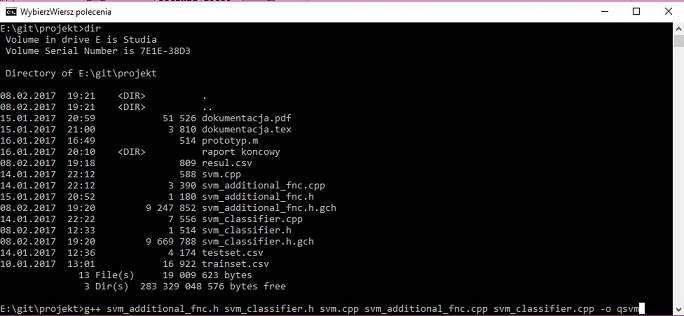
\includegraphics[width=4.50in, height=1.32in]{kompilacja.jpg} \textit \caption{Przykład wywoływania programu w kompilatorze g++ na systemie operacyjnym Microsoft Windows 10 (opracowanie własne).} \else 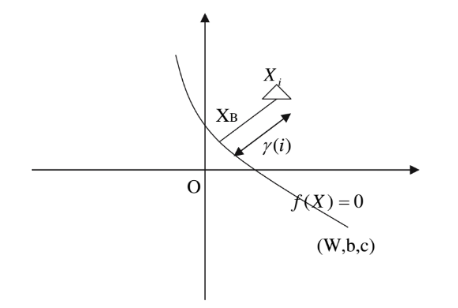
\includegraphics{3.ps} \fi \end{center} \end{figure}


\noindent Uruchomienie programu qsvm.exe rozpoczyna on działanie na próbkach trainset.csv oraz testset.csv i wyświetla on numer iteracji programu oraz Error rate podczas poszczególnych iteracji (poniższy rysunek). 

\begin{figure}[h] \begin{center} \ifpdf 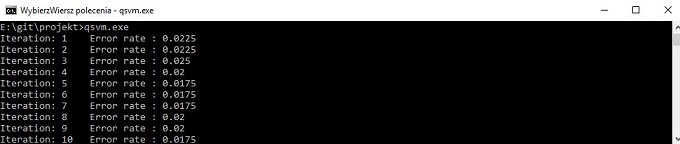
\includegraphics[width=4.50in, height=1.32in]{wywolanie.jpg} \textit \caption{Wyświetlenie numeru iteracji oraz Error rate (opracowanie własne).} \else 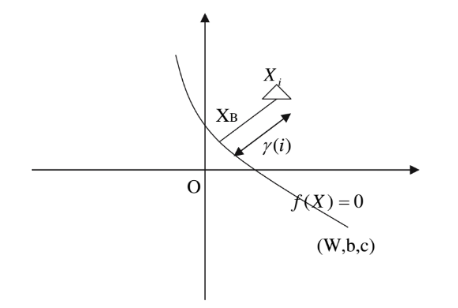
\includegraphics{3.ps} \fi \end{center} \end{figure}



\noindent Efekt klasyfikacji wyświetlany po zakończeniu programu -- etykiety próbek dla testset.csv oraz dokładność klasyfikacji i czasy treningu oraz predykcji (Rysunek 6).

\begin{figure}[h] \begin{center} \ifpdf 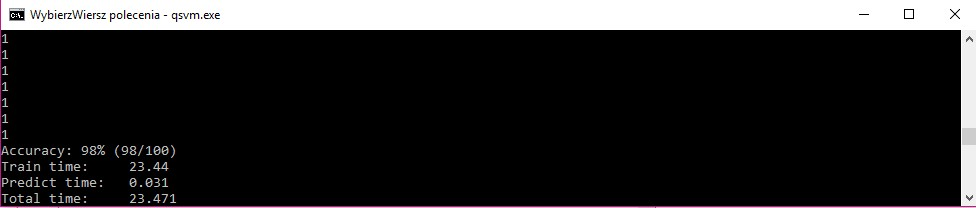
\includegraphics[width=4.50in, height=1.32in]{results.jpg} \textit \caption{Dane zwracane przez program po zakończeniu klasyfikacji (opracowanie własne).} \else 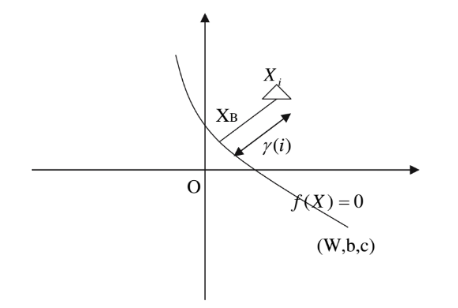
\includegraphics{3.ps} \fi \end{center} \end{figure}



\section{Badania eksperymentalne} 

\noindent W tej części przedstawimy rezulataty badań eksperymentalnych nad QSVM metodą SMO.


\subsection{Zbiór Iris}


\noindent Do wstępnego określenia skuteczności klasyfikacji zaimplementowanego rozwiązania zastosowano zbiór próbek ,,iris'' opisujący 150 przykładów należących do jednej z trzech klas będących różnymi typami rośliny irysów. Każdy typ irysa reprezentowany jest przez 50 przykładów opisanych przez 4 atrybuty określające wymiary składowych kwiatów. 

\noindent Pierwotna wersja klasyfikatora SVM odnosi się do dwóch klas. Istnieją metody pozwalające osiągnąć wieloklasową maszynę wektorów nośnych, jednak jest to związane z użyciem wielokrotnej klasyfikacji. Występują dwa podejścia rozwiązania problemu wieloklasowości maszyny wektorów nośnych:

\noindent \textit{- one against all}- zakłada stworzenie liczby klasyfikatorów równą liczbie klas. Każdy klasyfikator ma zbiór uczący podzielony na dwie części. Jedna część składa się ze zbioru uczącego jednej klasy, a druga złożona jest z pozostałych klas. Konkretna analizowana próbka poddawana jest klasyfikacji we wszystkich klasyfikatorach. Za wynik uważana jest klasa zwracająca maksymalny wynik[6].

\noindent - \textit{one against one }- polega na stworzeniu wszystkich N możliwych kombinacji dwuelementowych wszystkich k klas, czyli . Dane uczące każdego klasyfikatora zawierają dwie klasy. Wynikiem tego algorytmu, czyli określeniem przynależności do klasy jest największa liczba klasyfikacji do danej klasy ze wszystkich klasyfikatorów [7].

\noindent 

\noindent W tym przypadku wykorzystano metodę \textit{one against one}, ze wszystkich próbek stworzono po 3 zbiory uczące (80 próbek) oraz testowe (20 próbek ). Poniżej przedstawiono osiągnięte wyniki.

 \textit{Tabela 1. Wyniki klasyfikacji dla zbioru Iris}
 \newline
\begin{tabular} {|p{2.1in}|p{2.1in}|} \hline 
Zbiór próbek  & Osiągnięte wyniki \\ \hline 
Setosa + versicolor & Accuracy: 100\% (20/20)\newline Train time:     0.059\newline Predict time:   0.037\newline Total time:     0.096 \\ \hline 
Versicolor + virginica & Accuracy: 100\% (20/20)\newline Train time:     1.728\newline Predict time:   0.016\newline Total time:     1.744 \\ \hline 
Setosa + virginica & Accuracy: 100\% (20/20)\newline Train time:     0.009\newline Predict time:   0.019\newline Total time:     0.028 \\ \hline 
\end{tabular}



\noindent Na podstawie uzyskanych wyników można stwierdzić, że klasyfikator działa prawidłowo, ma on 100 \% skuteczności. Łatwo jest również zauważyć, iż dla zestawu próbek versicolor +  virginica czas train time jest najdłuższy. Tym samymm predict time jest najkrótszy co świadczy o tym, iż próbki zostały w odpowiedni sposób wytrenowane i dzięki temu klasyfikacja ich jest szybka. Dla zestawu próbek setosa + versicolor czas predict time jest najdłuższy. Moża stwierdzić, że algorytm w sposób najszybszy potraktował zestaw próbek setosa+virginica. 

\noindent 

\noindent 

\subsection{Wykorzystanie klasyfikatora do rozpoznawania uderzeń serca}

\noindent Każdy z klasyfikatorów wykonanych w ramach projektów grupy C testowane były przy pomocy dwóch określonych zbiorów danych, zawierających w sobie cechy opisujące uderzenia serca, w celu uwiarygodnienia porównania między sobą klasyfikatorów. W obu grupach uderzenia zostały podzielone na dwie klasy: uderzenia V, określające uderzenia wygenerowane w obrębie komory, zaliczane do patologicznych oraz uderzenia N -$>$ reprezentujące normalna, poprawna prace serca.

\subsubsection{ Zbiór danych 1}

\noindent Pierwszy zbiór danych składał się z pięciu cech opisujących uderzenia serca, bazując na interwałach RR ( kolejne szczyty zespołów QRS) . Do wyznaczenia zbioru próbek wykorzystano sygnały znajdujące się w bazie danych MIT-BIH (Massachussetts Institute of Technology -- Beth Israel Hospital) -- standardowa arytmiczna baza danych wykorzystano sygnały 228.dat oraz 100.dat .

\noindent Wykorzystane cechy : 

\begin{enumerate}
\item  \textbf{Pre interval} RR - odległość miedzy aktualnym uderzeniem serca(analizowanym), a poprzednim uderzeniem serca,

\item  \textbf{Post inreval RR} - odległość miedzy analizowanym uderzenie serca a kolejnym uderzeniem,

\item  \textbf{Average RR} - średnia długość interwału RR dla całego analizowanego sygnału,

\item  \textbf{Ratio1} - stosunek pre RR interval do post RR interval,

\item  \textbf{Ratio2 }- stosunek per interwalu do Avarage RR.
\end{enumerate}

\noindent Uzyskane próbki podzielono na dwie części w stosunku 4:1, 400 próbek treningowych oraz 100 próbek testowych. Poniżej w tabeli przedstawiono uzyskane wyniki rozpoznania próbek odpowiednio do klas N oraz V.

\textit{Tabela 2. Tabela uzyskanych wyników dla zbioru danych 1}
\newline
\begin{tabular}{|p{1.1in}|p{1.1in}|p{1.1in}|p{1.1in}|} \hline 
 & Dobrze rozpoznane & \'{Z}le rozpoznane & Całość klasy  \\ \hline 
Uderzenia N & 48 & 2 & 0,99 \\ \hline 
Uderzenia V & 49 & 2 & 0,98 \\ \hline 
\multicolumn{3}{|p{1in}|}{Skuteczność rozpoznawania [\%]:} & 97 \\ \hline 
\end{tabular}



\noindent Proces uczenia trwał dla systemu QSVM 24780 ms, natomiast czas klasyfikacji 59 ms, długa ilość uczenia systemu spowodowana jest skomplikowanym algorytmem SMO i konieczności przejścia dużej liczby iteracji do zoptymalizowania dwóch punktów. Można uznać, że skuteczność klasyfikacji uzyskano na wysokim poziomie, 97 \%. 

\noindent Dla uzyskanych wyników również wyliczono czułość ( ang. Sensitivity), wyliczona z poniższego wzoru:
 $$
sensitivity = \frac{TP}{TP + FN}
$$

\noindent TP (ang. Truepositive) -- liczba poprawnie sklasyfikowanych przykładów wybranej klasy,

\noindent FN ( ang. Falsenegative) -- liczba błędnie sklasyfikowanych przykładów z tej klasy,

\noindent Czułość klasyfikacji wynosi 96 \%. Wyznaczono również specyficzność klasyfikacji ( ang. Specifity) może być wyznaczona jako stosunek TN do sumy FP oraz TN.

 $$
specifity = \frac{TN}{FP + TN}
$$
\\
TN ($ang. true negative$) - liczba przykładów poprawnie nie przydzielonych do wybranej klasy (poprawnie odrzuconych z $ang. correct rejection$)\\
\\
FP ($ang. false positive$) - liczba przykładów błędnie przydzielonych do wybranej klasy, podczas gdy w rzeczywistości do niej nie należą ($ang. false alarm$)\\

\noindent Specyficzność tej klasyfikacji wynosi również 96 \%. 

\subsubsection{Zbiór danych 2} 

\noindent Drugi zbiór danych również reprezentowała 5 cech sygnału z uderzeniami serca. Próbki podzielone również były w tak samo liczne grupy treningowe i testową. W skład grupy testowej wchodziło 100 próbek, natomiast do treningowej wchodziło 400 próbek.

\noindent Zbiór danych numer 2 zawierał w sobie cechy :

\begin{enumerate}
\item  Stosunek pola do obwodu (współczynnik Malinowskiej) 
 \\$p_1 = \frac{\sum_{k=1}^{N} s[k]}{\sum_{k=2}^{N} s[k]-s[k-1]}$

\item  Wartość międzyszczytowa
\\$p_2 = \frac{\max_{k \in <1,N>} s[k]}{\min_{k \in <1,N>} s[k]}$

\item  Procent próbek sygnału, które są ujemne    \\$p_3 = 100\% * \frac{\sum_{k=1}^{N} u[k]}{N}$ 

\item  Stosunek maksymalnej prędkości do maksymalnej amplitudy 
\\$p_4 = \frac{\max_{k \in <3,N>} s[k]-s[k-2]+2s[k-1]}{|\max_{k \in <1,N>} s[k] - \min_{k \in <1,N>} s[k]|}$

\item  Stosunek liczby próbek sygnału, których prędkość przekracza 40\% maksymalnej prędkości obserwowanej 
\\$p_5 = \frac{\sum_{k=1}^{N} g[k]}{N}$

\end{enumerate}
\textit{Tabela 3. Wynik klasyfikacji dla zbioru 2}
\newline
\begin{tabular}{|p{1.2in}|p{1.0in}|p{1.0in}|p{1.0in}|} \hline 
 & Dobrze rozpoznane & \'{Z}le rozpoznane & Całość klasy  \\ \hline 
Uderzenia N & 76 & 0 & 1 \\ \hline 
Uderzenia V & 22 & 2 & 0,96 \\ \hline 
\multicolumn{3}{|p{1in}|}{Skuteczność klasyfikacji [\%] } & 98 \\ \hline 
\end{tabular}



\noindent Dla klasyfikacji tego zbioru danych również wyznaczono wartość czułości i skuteczności klasyfikacji analogiczną metodą przedstawioną w ostatnim podrozdziale. Czułość w przypadku tego zbioru danych osiągnęła maksymalne 100 \%, a specyficzność 91,6 \%.

\noindent Accuracy: 98\% (98/100)

\noindent Train time:     22.943

\noindent Predict time:   0.01

\noindent Total time:     22.953

\noindent Uczenie klasyfikatora zajęło 22.953 s, natomiast czas klasyfikacji 0.01 s, jest to znacznie niższa liczba prawdopodobnie spowodowana zastosowaniem innych cech charakteryzujących sygnał. 

\noindent Różna ilość cech wykorzystanych do klasyfikacji.

\noindent 

\noindent 

\subsubsection{Porównanie klasyfikacji z różna ilością cech} 
\noindent W celu określenia działania klasyfikacji przetestowano również testowanie klasyfikatora z różną ilością cech określających sygnał. Kolejno z 1, 2, 3, 4 cechami w próbkach uczących i testowych. Poniżej przedstawiono w tabeli uzyskane wyniki.\\
\textit{ Tabela 4. Porównanie klasyfikacji dla róznej ilości cech}
\newline
\begin{tabular}{|p{0.25\linewidth}|p{0.8in}|p{0.8in}|p{0.8in}|p{0.8in}|} \hline 
 & \textbf{1 cecha} & \textbf{2 cechy} & \textbf{3 cechy} & \textbf{4 cechy} \\ \hline 
\textbf{Skuteczność rozpoznawania [\%]} & 98 \% & 98 \% & 98 \% & 98 \% \\ \hline 
\textbf{Czas uczenia [s]} & 43.1 & 10.427 & 17.613 & 25.13 \\ \hline 
\textbf{Czas klasyfikacji [s]} & 0.009 & 0.011 & 0.009 & 0.011 \\ \hline 
\textbf{Czułość} & 100 & 100 & 100 & 100 \\ \hline 
\textbf{Specyficzność} & 91,6 & 91,6 & 91,6 & 91,6 \\ \hline 
\end{tabular}\\



\noindent Z powyższych uzyskanych wyników można zauważyć, że skuteczność klasyfikacji jest na tym samym poziomie bez względu na ilość zastosowanych cech. Również analizując uzyskane wyniki niepoprawnie zostały sklasyfikowane te same próbki w każdym przypadku. Jednak przypadki między sobą różnią się długością czasu klasyfikacji oraz ilością koniecznych iteracji do nauczenia się programu. Z rosnącą ilością cech opisujących sygnały czas klasyfikacji ma tendencję malejącą do 3 cech, a następnie dla 4 cech i 5 do około 22-25 s. Dla jednej cechy czas uczenia był najdłuższy zajął aż 43.1 sekundy. Najszybszym nauczeniem charakteryzował się zbiór danych z dwoma cechami oraz trzema. Oznacza to, ze dla klasyfikatora należy wybrać pośrednią liczbę cech (najlepiej zachowuje się przy niezbyt niskiej i niezbyt wysokiej liczbie próbek). 

\noindent 

\noindent 


\newpage
\section{Porównanie wyników różnych klasyfikatorów}
W tym rozdziale przedstawimy różnicę w wynikach uzyskanych dla wszytskich klasyfikatorów: k-Neraest Neighbours (kNN), Extended Nerest Neighbours (eNN), Radial Basis Function Kernel (RBF SVM), klasyfikator Bayesa, Linear SVM, Quadratic SVM.
\subsection{Zbiór danych 1}
Poniżej przedstawiono wyniki uzyskane podczas klasyfikacji zbioru danych nr 1 przez wszystkie klasyfikatory. Wyznaczono takie parametry jak: skuteczność klasyfikacji, czas uczenia, czas klasyfikacji, czułość oraz specyficzność.\\
\textit{Tabel 6. Wyniki klasyfikacji wszystkich użytych klasyfikatorów dla zbioru 1}
\newline
\begin{tabular}{|p{0.25\linewidth}|p{0.48in}|p{0.48in}|p{0.48in}|p{0.48in}|p{0.48in}|p{0.48in}|p{0.48in}|} \hline 
 & \textbf{kNN} & \textbf{ENN} & \textbf{Linear SVM} & \textbf{SVM + RBF} & \textbf{Naive Baye} & \textbf{LDA} & \textbf{QSVM} \\ \hline 
\textbf{Skuteczność klasyfikacji [\%]}  \textbf{} &99  & 99 & 99.7261 & 92.8789 & 99.8783 & 99.73 & 97 \\ \hline 
\textbf{Czas uczenia [ms]} & brak & brak & 25003 & 7865 & 22.0936 & 3 & 24780 \\ \hline 
\textbf{Czas klasyfikacji [ms]} & 3563 & 36328 & 26 & 1961 & 1925 & 13 & 59 \\ \hline 
\textbf{Czu{\l}o\'{s}\'{c}} & 99 & 99 & 99.7129 & 92.5678 & 99.9681 & 98.68 & 96 \\ \hline 
\textbf{Specyficzność} & 100 & 100 & 100 & 100 & 98.0132 & 95.83 & 96 \\ \hline 
\end{tabular}
\newline

Badany klasyfikator QSVM w porównaniu do innych badanych klasyfikatorów na tym zbiorze danych zajął 6 miejsce mimo osiągnięcia dosyć wysokiego wyniku poprawnego sklasyfikowania uderzenia serca, 97 procent. Z tabeli wynika, że QSVM zalicza się do klasyfikatorów długo uczących się, osiągnęło zbliżone wyniki do pozostałych padanych  SVM z innymi jądrami, więc QSVM pod względem czasu uczenia jest jednym z gorszych klasyfikatorów. Jednak zaletą SVM jest szybki czas klasyfikacji, co też widać z powyższych danych, że QSVM jest trzeci najszybszy w klasyfikacji.  \\

\scalebox{0.9}{
 \begin{bchart}[max=100, unit=\%]
 \bcbar[label={Klasyfikatory}, text=kNN,
 color=white]{99}
 \bcbar[text=ENN, color=gray!50]{99}
 \bcbar[text=linear SVM, color=gray!10]{99.7261}
\bcbar[text=SVM + RBF, color=gray!50]{92.8789}
 \bcbar[text=Naive Baye, color=gray!80]{99.8783}
 \bcbar[text=LDA, color=gray!80]{99.73}
 \bcbar[text=QSVM, color=gray!80]{97}
 \bcxlabel{\% Skutecznosc}
 \end{bchart}
 }
 \newline
 \textit{Wykres 1. Wykres procentowy przedstawiający skuteczność klasyfikacji wszystkich użytych klasyfikatorów dla zbioru 1}
\newline

\subsection{Zbiór danych 2}
\textit{Tabel 5. Wyniki klasyfikacji wszystkich użytych klasyfikatorów dla zbioru 2}
\newline
\begin{tabular}{|p{0.25\linewidth}|p{0.45in}|p{0.45in}|p{0.45in}|p{0.45in}|p{0.45in}|p{0.45in}|p{0.45in}|} \hline 
 & \textbf{kNN} & \textbf{ENN} & \textbf{Linear SVM} & \textbf{SVM + RBF} & \textbf{Naive Baye} & \textbf{LDA} & \textbf{QSVM} \\ \hline 
\textbf{Skuteczność klasyfikacji [\%]}  \textbf{} &98  & 98 &76 & 99 & 96 & 98 & 98 \\ \hline 
\textbf{Czas uczenia [ms]} & brak & brak & 8517 & 13481 & 21.9 & 15 & 22953 \\ \hline 
\textbf{Czas klasyfikacji [ms]} & 109 &1094 & 1 & 79 & 29.29 & 1 & 10 \\ \hline 
\textbf{Czułość} & 97 & 100 & 100 & 100 & 97.36 & 99.78 & 100 \\ \hline 
\textbf{Specyficzność} & 100 & 92 & 4 & 96 & 92 & 98.67 & 91.6 \\ \hline 
\end{tabular}
\newline
Biorąc pod uwagę skuteczność klasyfikacji dla zbioru 2 jedynie klasyfikator SVM + RBF wykazał lepszy wynik. QSVM razem z kNN, ENN i LDA rozpoznaje na poziomie 98. Jak już wspomniano czas uczenia dla tego klasyfikatora jest długi. Warto jednak tu podkreślić, że czas klasyfikacji dzięki dobremu wytreniowaniu zbioru jest stosunkowo krótki. 
\newpage
\scalebox{0.9}{
 \begin{bchart}[max=100, unit=\%]
 \bcbar[label={Klasyfikatory}, text=kNN,
 color=white]{98}
 \bcbar[text=ENN, color=gray!50]{98}
 \bcbar[text=linear SVM, color=gray!10]{76}
\bcbar[text=SVM + RBF, color=gray!50]{99}
 \bcbar[text=Naive Baye, color=gray!80]{96}
 \bcbar[text=LDA, color=gray!80]{98}
 \bcbar[text=QSVM, color=gray!80]{98}
 \bcxlabel{\% Skutecznosc}
 \end{bchart}
 }
  \newline
 \textit{Wykres 2. Wykres procentowy przedstawiający skuteczność klasyfikacji wszystkich użytych klasyfikatorów dla zbioru 2}
 
 
 \subsection{Wnioski}
 QSVM na tle innych użytych klasyfikatorów kNN, ENN, linear SVM, SVM + RBF, Naive Baye i LDA wykazał się stosunkowo dobrą skutecznościa. Dla zbioru danych 1 wynik ten jest znacznie gorszy w porównaniu do liniowego odpowiednika SVM, który to osiągnął skuteczność prawie stu procentową. Czas uczenia był porównywalny do QSVM jednak czas klasyfikacji był już krótszy. Warto tu podkreślić, że metoda SVM dobrze sobie radzi z nadmiernym dopasowaniem danych. Dla zbioru 2 skuteczność dla większości klasyfikatorów była porównywalna. 
 \newline QSVM charakteryzuje stosunkowo dlugi czas uczenia. Związane jest to z faktem, iż metoda ta wymaga użycia Quadratic Programming co dla dużej ilości danych powoduje problem z szybkością działania algorytmu. W celu uniknięcia tego stosuję się opisaną na początku pracy metodę dekompozycji dzięki, której  zbiór rozpatrywany jest w kilku etapach. 
\newpage

\begin{thebibliography}{10}
	
	\bibitem{platt}
	Platt John
	\textit{Sequential Minimal Optimalization: A fast Algorithm for Ftaining Support Vector Machines} 
	Microsoft Reasearch, Technical Report, MSR-TR-98-12, 1998
	\bibitem{mgr}
	Marcin Orchel
	\textit{Klasyfikacja danych wielowymiarowych algorytmami SVM} 
	Praca magisterska, Akademia Górniczo-Hutnicza, Wydział Elektrotechniki Automatyki Informatyki i Inżynierii Biomedycznej
	\bibitem{simplified}
	\textit{The Simplified SMO Algorithm} 
	 CS229 Machine Learning, Stanford
	 \bibitem{iowa}
	Vasant Honavar 
	\textit{Sequential MinimalOptimalization for SVM} 
	Iowa State University, Computer Science Department 
 \bibitem{blog}
	Juan Miguel 
	\textit{[SVM Matlab code implementation] SMO (Sequential Minimal Optimization) and Quadratic Programming explained} 
	http://laid.delanover.com/svm-matlab-code-implementation-smo-sequential-minimal-optimization-and-quadratic-programming-explained/
	\bibitem{kmiec}Marcin Kmieć
	\textit{Wykrywanie niebezpiecznych przedmiotów w automatycznie
analizowanych sekwencjach wideo} 
	  Akademia Górniczo-Hutnicza, Kraków
	  \bibitem{sieci}Piotr Walendowski
	\textit{Zastosowanie sieci neuronowych typu SVM do
rozpoznawania mowy.} 
	  Politechnika Wrocławska, Wydział Elektroniki, Wrocław
\end{thebibliography}

\end{enumerate}

\end{document}







